\chapter{Minh hoạ kết quả suy luận của cử chỉ}
\label{Appendix3}

\section{So sánh giữa cử chỉ groundtruth và cử chỉ dự đoán}


\begin{center}
\centering
\href{https://youtu.be/22lNm2tvmrk}{% Replace with your YouTube URL
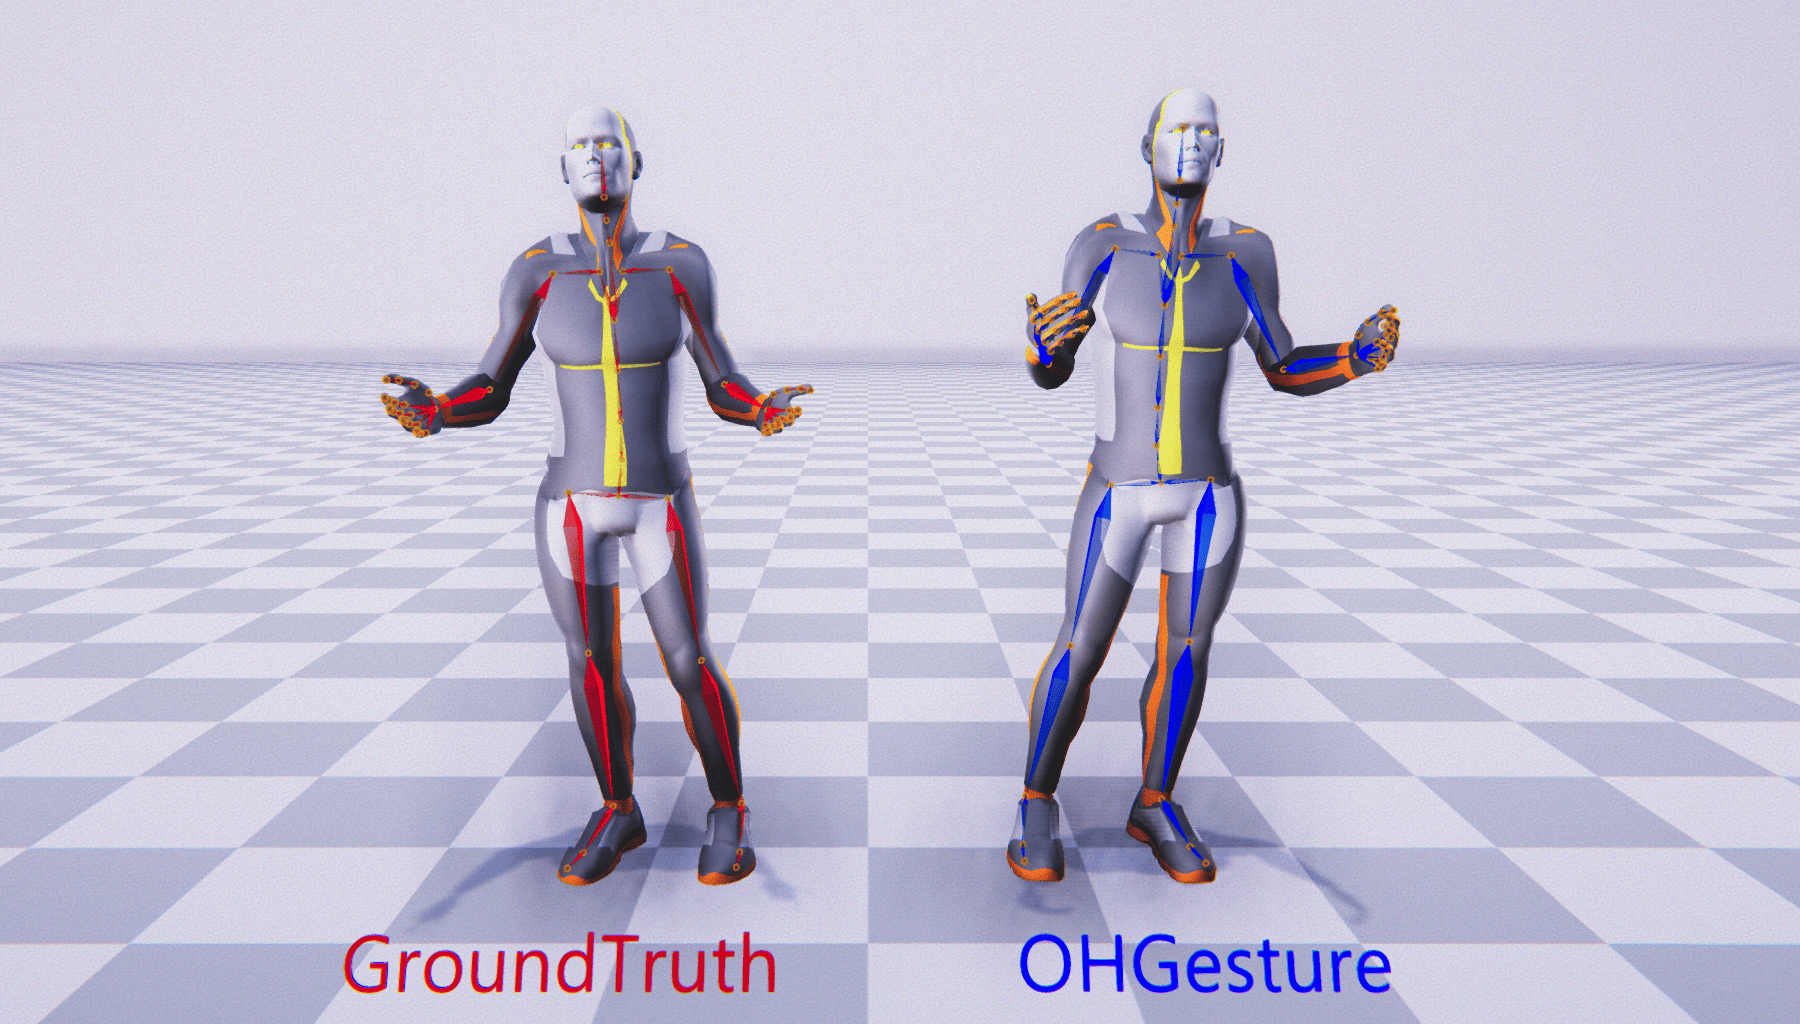
\includegraphics[width=\textwidth]{GroundTruthCompare}}
{\tiny Click vào ảnh để xem video}
\end{center}

Kết quả cử chỉ ground truth và cử chỉ dự đoán của mô hình ở frame $3821$ dự đoán trên mẫu âm thanh $\texttt{003\_Neutral\_2\_x\_1\_0}$

\section{Minh học việc sinh cử chỉ với âm thanh nằm ngoài tập huấn luyện}

{
	\begin{center}
		\centering
		\href{https://www.youtube.com/watch?v=B6nv1kQmi-Q}{% Replace with your YouTube URL
		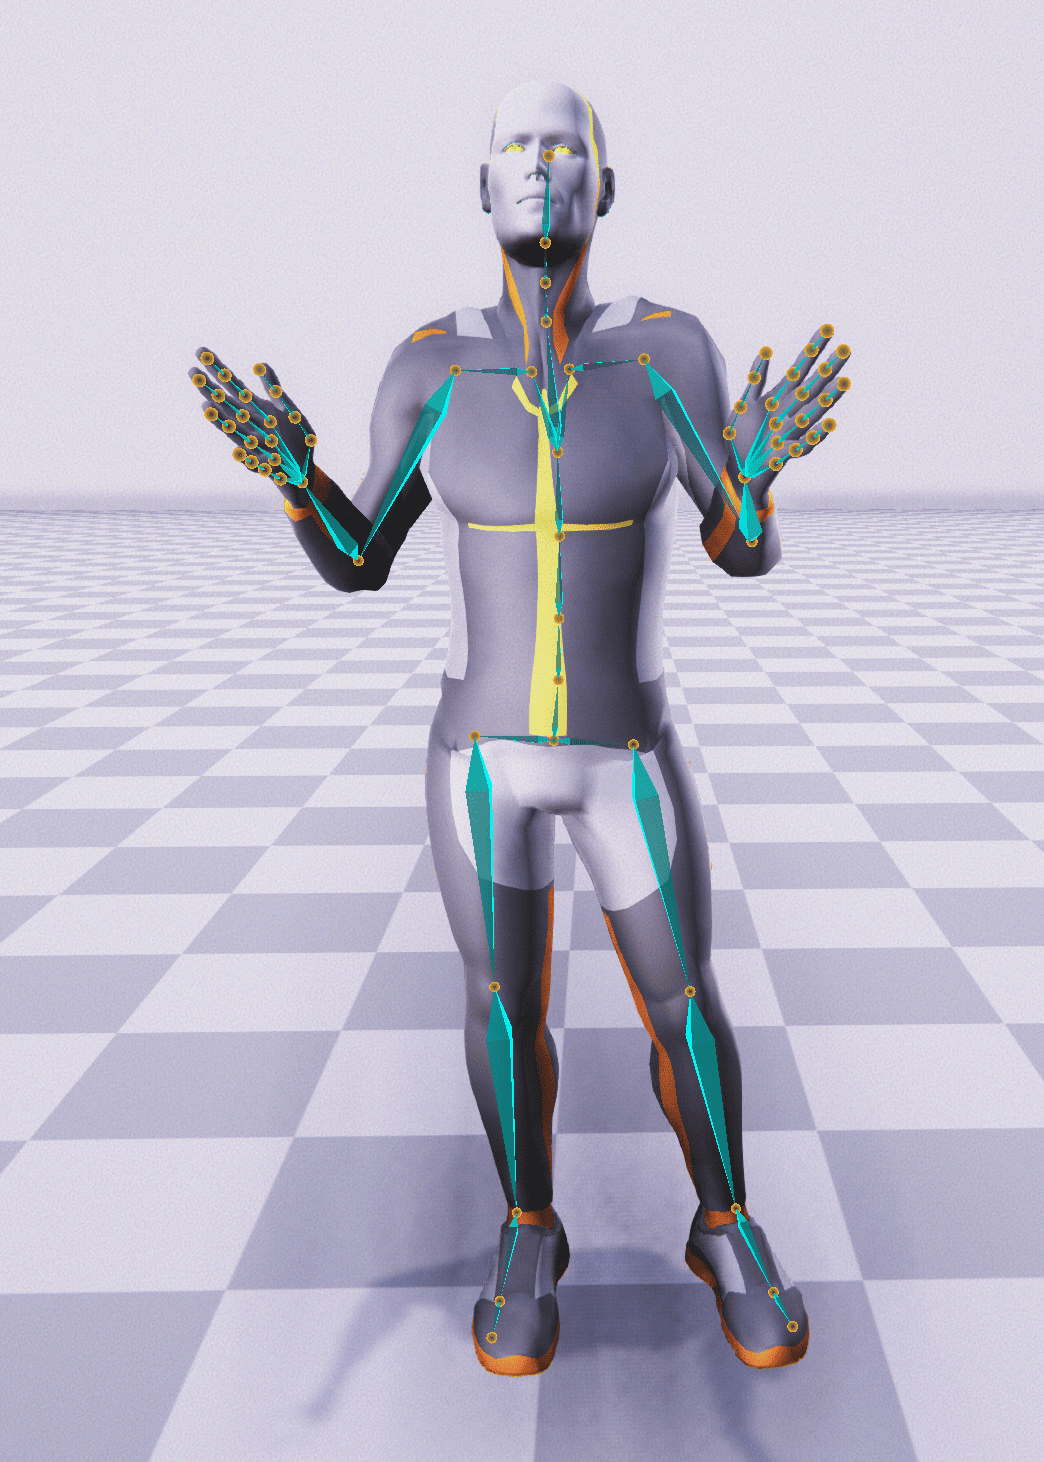
\includegraphics[width=0.4\textwidth]{StevenJob}}
		
		{\tiny Click vào ảnh để xem video}
	\end{center}

}

Minh hoạ sinh cử chỉ tương ứng với âm thanh của Steven Job



\section{Minh học chuyển động của nhân vật}

\begin{center}
{
	\centering
	\href{https://www.youtube.com/watch?v=9IIIZP3EJLg}{% Replace with your YouTube URL
	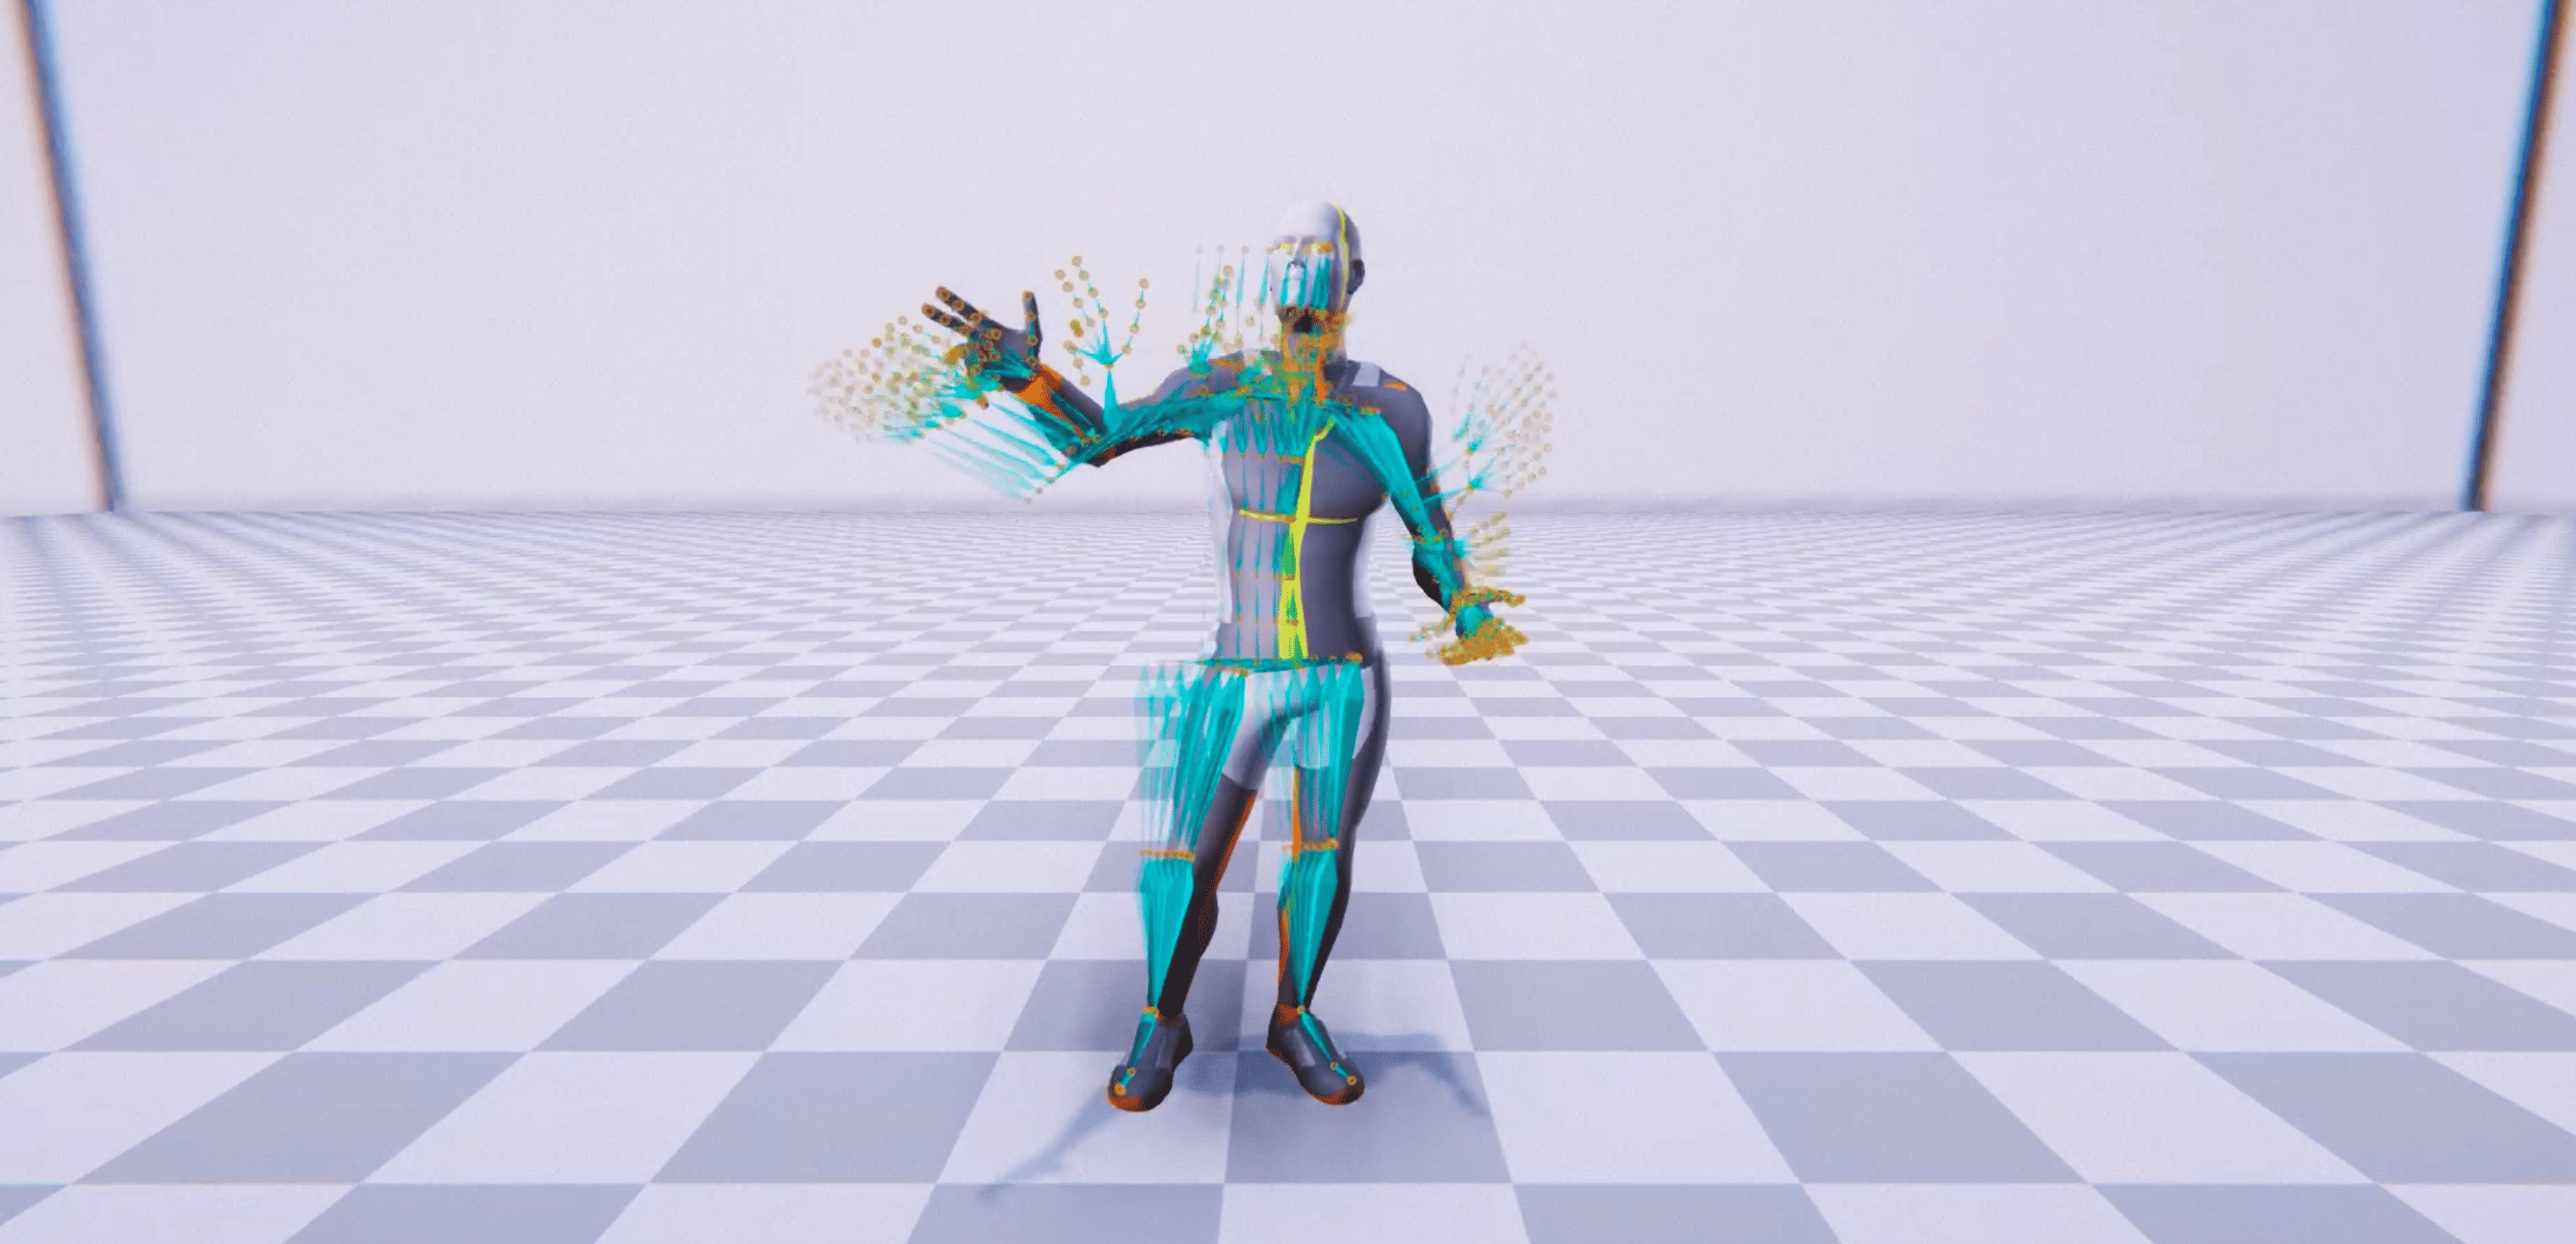
\includegraphics[width=0.8\textwidth]{DemoMotionGesture}}
	
	{\tiny Click vào ảnh để xem video}
}
\end{center}
Minh hoạ cử chỉ được lấy 6 khung hình phía trước và 6 khung hình phía sau của cử chỉ.